% Journal-style manuscript: lifecycle portfolio allocation (DP + RL)
% Compile from the project/ directory: pdflatex lifecycle_rl_paper.tex
\documentclass[11pt,a4paper]{article}

\usepackage[margin=1in]{geometry}
\usepackage{amsmath,amssymb,amsfonts}
\usepackage{booktabs}
\usepackage{graphicx}
\usepackage{hyperref}
\usepackage{natbib}
\usepackage{authblk}
\usepackage{caption}

\hypersetup{colorlinks=true,linkcolor=blue,citecolor=blue,urlcolor=blue}

\title{Reinforcement Learning for Lifecycle Portfolio Allocation:\\
From Exact Dynamic Programming to Function Approximation}

\author[1]{Patrick Flanagan}
\author[1]{Jack Zhang}
\author[1]{Jeffrey Xue}
\affil[1]{Stanford University, CME 241 --- Reinforcement Learning for Stochastic Control in Finance (Winter 2026)}

\date{\today}

\begin{document}
\maketitle

\begin{abstract}
We study finite-horizon lifecycle consumption and portfolio choice with stochastic labor income and market regimes, maximizing discounted constant relative risk aversion (CRRA) utility of consumption plus a terminal bequest. A tractable discrete-state formulation is solved exactly by backward dynamic programming (DP), validating objectives and baselines. A scaled ``realistic'' parameterization exhibits a roughly $119\times$ increase in DP table size, motivating reinforcement learning (RL). We implement a Gymnasium-style simulator and four agents: linear $Q$-learning, SARSA with linear function approximation, Dueling Deep $Q$-Networks (DQN), and Proximal Policy Optimization (PPO). Engineering fixes---consistent penalization of zero consumption, correct training dispatch for on-line versus replay-based updates, randomized initial states, and architecture choices---are essential for learning non-degenerate, state-dependent policies. Monte Carlo evaluation on 2{,}000 simulated lifetimes shows all RL methods outperform static $60/40$, equal-weight, and glidepath rules on expected utility, with Dueling DQN achieving the highest mean utility among RL agents while linear methods offer interpretability and orders-of-magnitude faster training.
\end{abstract}

\noindent\textbf{Keywords:} lifecycle portfolio choice; dynamic programming; reinforcement learning; CRRA utility; SARSA; DQN; PPO

\section{Introduction}

Households approaching retirement face a joint problem: how much to consume each period versus save, and how to allocate savings across risky and safe assets, while income and investment opportunities evolve stochastically. Target-date funds and rules of thumb (e.g., static stock--bond mixes or deterministic glidepaths) are widely used but need not optimize a well-specified welfare objective.

This paper documents a two-stage computational project. \textbf{Phase~2} embeds the problem in a finite Markov decision process (MDP) with a coarse wealth grid and solves it \emph{exactly} by backward induction, comparing the optimal policy to simple benchmarks. \textbf{Phase~3} enlarges the horizon, the number of income and regime states, and the fineness of the action grid; exact tabular DP becomes impractical. We instead learn policies with RL, using function approximation over a low-dimensional state feature vector and a discrete joint action space for consumption fraction and portfolio weights.

Our contributions are: (i)~a reproducible DP baseline and curse-of-dimensionality accounting; (ii)~a unified open-source environment (\texttt{PortfolioEnv}) with economically interpretable rewards $\beta^t u(c_t)$; (iii)~four RL algorithms spanning off-policy and on-policy, linear and deep; and (iv)~an explicit discussion of implementation pitfalls (reward bugs, training dispatch errors, evaluation metrics) that dominate short-horizon applied RL projects.

\section{Related work}

Lifecycle models with portfolio choice are central in macro-finance \citep{samuelson1969lifetime,merton1969lifetime}. Exact solutions are typically available only in continuous-time special cases; realistic models require numerical methods. Approximate dynamic programming and fitted value iteration are standard in economics \citep{judd1998numerical}. Deep RL has been applied to portfolio management and related control problems \citep{jiang2017cryptocurrency}; our setting emphasizes consumption--portfolio interaction and finite horizons with explicit discounting in the reward. Algorithmically we build on $Q$-learning and SARSA \citep{sutton2018reinforcement}, DQN and Dueling architectures \citep{mnih2015human,wang2016dueling}, and PPO \citep{schulman2017proximal}.

\section{Problem formulation}

\subsection{MDP structure}

Let time $t \in \{0,\ldots,T-1\}$. The state is $s_t = (t, W_t, y_t, z_t)$: calendar time, wealth $W_t \ge 0$, discrete income state $y_t$, and discrete market regime $z_t$. The action is a pair $(\alpha_t, \mathbf{w}_t)$: consumption fraction $\alpha_t \in [0,1]$ (chosen from a finite grid) and portfolio weights $\mathbf{w}_t$ over stocks, bonds, and cash (simplex, discretized). Consumption is $c_t = \alpha_t W_t$; savings are $(1-\alpha_t)W_t$. Gross asset returns $\mathbf{R}_t$ are drawn from a finite set whose distribution depends on $z_t$. Next-period wealth is
\begin{equation}
  W_{t+1} = \bigl(W_t - c_t\bigr)\, (\mathbf{w}_t^\top \mathbf{R}_t) + \text{income}(y_{t+1}),
\end{equation}
with $y_{t+1}$ and $z_{t+1}$ following Markov transitions. The objective is
\begin{equation}
  \max_\pi \; \mathbb{E}_\pi \left[ \sum_{t=0}^{T-1} \beta^t u(c_t) + \beta^T u(W_T) \right],
\end{equation}
with CRRA utility $u(c) = c^{1-\gamma}/(1-\gamma)$, $\gamma = 2$, so $u(c) = -1/c$ for $c>0$. Near-zero consumption is penalized by a large negative surrogate in code for numerical stability (aligned with DP treating zero consumption as infeasible).

\subsection{Phase~2: exact DP (small scale)}

We discretize wealth on 121 grid points, use two income and two regime states, $T=25$, $\beta=0.96$, $\gamma=2$, 11 consumption fractions ($0\%, 2\%, \ldots, 20\%$), and 15 allocations (25\% increments). There are $165$ actions per state and about $2.0\times 10^6$ DP cells per full backward pass; the solver runs in under one second. Terminal values are $V_T(W)=u(W)$; for $t<T$ we maximize over actions and expectation over income, regime, and return shocks, with interpolation on the wealth grid where needed.

\subsection{Phase~3: scaled MDP and RL interface}

Phase~3 uses $T=40$, three income levels $\{3,10,25\}$, three regimes \{bear, normal, bull\}, transition matrices as in the codebase, three return scenarios per regime, 11 consumption fractions, and 21 three-asset allocations (20\% increments), yielding \textbf{231} atomic actions. Wealth is treated as continuous within $[W_{\min}, W_{\max}]$ with $W_{\min}=0.01$, $W_{\max}=800$, and initial evaluation wealth $W_0=100$.

The environment maps the latent state to an \textbf{eight-dimensional} feature vector: normalized time $t/T$, normalized log wealth $\log W / \log W_{\max}$, one-hot$(y)$ (3), and one-hot$(z)$ (3). The step reward is $r_t = \beta^t u(c_t)$; at termination an additional $\beta^T u(W_T)$ is added. RL discount $\gamma_{\mathrm{RL}}$ is set to $1$ so that undiscounted return equals the economic objective; discounting is entirely in the reward.

Training uses \textbf{randomized resets}: log-uniform wealth in $[10,\,0.6\,W_{\max}]$, uniform random income and regime. This widens state coverage and is critical for state-dependent policies.

\section{Algorithms}

\subsection{\texorpdfstring{Linear $Q$-learning}{Linear Q-learning}}

We approximate $Q(s,a) \approx \mathbf{w}_a^\top \boldsymbol{\phi}(s)$ with shared features $\boldsymbol{\phi}(s) \in \mathbb{R}^{24}$: raw 8-D state, polynomials $(t^2, w^2, tw)$, interactions of normalized time and wealth with each of six categorical indicators, and a bias. There are $231\times 24 = 5544$ scalar weights. Updates are semi-gradient $Q$-learning with $\varepsilon$-greedy exploration. Hyperparameters: learning rate $\alpha=10^{-5}$, $\gamma_{\mathrm{RL}}=1$, $\varepsilon$ linearly from $1$ to $0.05$ over 8{,}000 episodes, 15{,}000 episodes total.

\subsection{SARSA}

The same linear architecture is trained on-policy: the TD target uses $Q(s',a')$ where $a'$ is the action that will be executed, enforced via a cached next-action mechanism. TD errors are clipped to $[-10,10]$ for stability under large negative utilities.

\subsection{Dueling DQN}

A neural network with trunk $8\to 256 \to 256$ (tanh) feeds a value head $256\to 1$ and an advantage head $256\to 231$, combined as $Q(s,a)=V(s)+A(s,a)-\frac{1}{|\mathcal{A}|}\sum_{a'}A(s,a')$ \citep{wang2016dueling}. Experience replay ($10^5$ transitions), target network updates every 200 steps, Huber loss, Adam learning rate $3\times 10^{-4}$, batch size 128, gradient clip norm 10.

\subsection{PPO}

Separate actor and critic MLPs ($8\to 256\to 256\to$ logits or scalar value), orthogonal initialization, rollout length 2048, GAE $\lambda=0.95$, clip $\epsilon=0.2$, entropy coefficient $0.05$, 10 epochs per rollout, minibatches of 128. Stochastic policy with scheduled exploration decay.

\subsection{Training infrastructure}

Agents declare \texttt{uses\_replay}: DQN and PPO call \texttt{store}/\texttt{train\_step}; linear $Q$ and SARSA call \texttt{update} each step. This avoids a subtle bug where a base-class \texttt{store} stub caused linear methods to never update.

\section{Implementation issues and remedies}

\textbf{Zero-consumption exploit.} Returning reward zero when $c=0$ made ``never consume'' optimal because $u(c)<0$ for all $c>0$ under $\gamma=2$. Rewards now always use the CRRA-based penalty for negligible consumption.

\textbf{Evaluation utility.} Monte Carlo utility accumulation must apply the same penalty; skipping zero-consumption periods had inflated reported utility for degenerate policies.

\textbf{Architectures.} PPO benefited from decoupled actor--critic networks; DQN benefited from the dueling head and larger width (256). Randomized initial states dominated other changes for visible state dependence in policies.

\section{Experiments}

We train each agent for 15{,}000 episodes. Evaluation uses 2{,}000 simulated paths starting at wealth $W_0=100$, medium income, and normal regime. Baselines are static $60/40$ stocks/bonds, equal thirds, and a linear stock glidepath $80\%\to 20\%$ with the remainder in bonds. Table~\ref{tab:main} reports mean discounted CRRA utility and terminal wealth moments; Table~\ref{tab:risk} summarizes risk-style metrics from the same simulations.

\begin{table}[htbp]
  \centering
  \caption{Monte Carlo evaluation (2{,}000 paths). Utility is expected total discounted CRRA objective; wealth statistics are terminal $W_T$.}
  \label{tab:main}
  \begin{tabular}{l r rrr r r}
    \toprule
    Strategy & $\mathbb{E}[U]$ & $\mathbb{E}[W_T]$ & Med$[W_T]$ & Std$[W_T]$ & $P_{10}[W_T]$ & $P_{90}[W_T]$ \\
    \midrule
    DQN & $-1.54$ & 115.3 & 107.2 & 51.8 & 57.9 & 185.5 \\
    Linear $Q$ & $-1.59$ & 96.0 & 86.6 & 33.8 & 59.8 & 144.2 \\
    SARSA & $-1.88$ & 99.1 & 93.3 & 35.3 & 58.1 & 149.9 \\
    PPO & $-1.95$ & 91.0 & 81.2 & 43.2 & 44.8 & 149.8 \\
    \midrule
    Static 60/40 & $-2.63$ & 487.3 & 470.1 & 166.1 & 281.0 & 747.3 \\
    Glidepath & $-2.63$ & 489.1 & 474.1 & 140.0 & 319.7 & 696.5 \\
    Equal $1/3$ & $-2.75$ & 407.8 & 396.1 & 112.4 & 270.5 & 564.4 \\
    \bottomrule
  \end{tabular}
\end{table}

\begin{table}[htbp]
  \centering
  \caption{Risk-style metrics (same simulations). Sharpe$(C)$ denotes a consumption-based Sharpe measure computed in the project pipeline.}
  \label{tab:risk}
  \begin{tabular}{l r r r}
    \toprule
    Strategy & Max drawdown (\%) & Sharpe$(C)$ & $\min W_T$ \\
    \midrule
    DQN & 60.4 & 26.53 & 18.3 \\
    Linear $Q$ & 54.0 & 18.30 & 33.2 \\
    SARSA & 57.1 & 10.25 & 24.9 \\
    PPO & 66.1 & 12.58 & 20.5 \\
    Static 60/40 & 23.8 & 2.65 & 98.4 \\
    \bottomrule
  \end{tabular}
\end{table}

\begin{figure}[htbp]
  \centering
  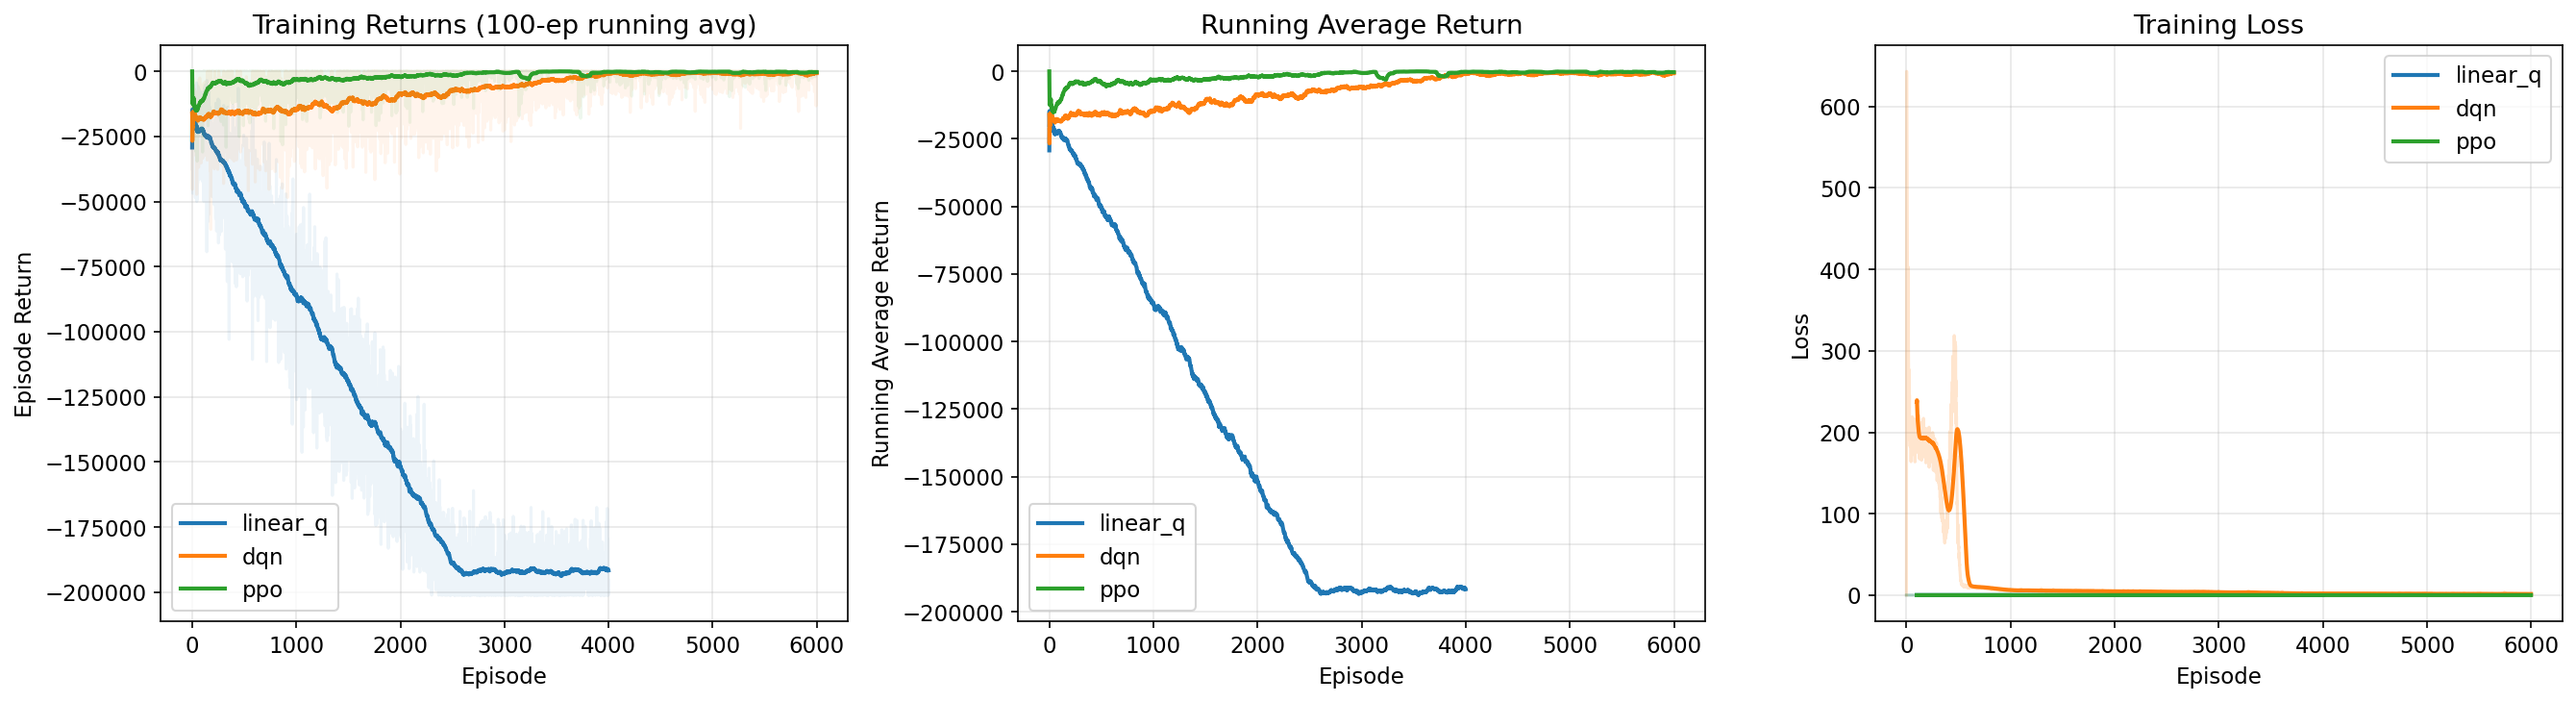
\includegraphics[width=0.95\textwidth]{phase3/plots/learning_curves.png}
  \caption{Training diagnostics (100-episode smoothed returns, running averages, and loss for applicable agents). PPO typically moves fastest in return space; DQN loss decreases as replay fills.}
  \label{fig:learn}
\end{figure}

\begin{figure}[htbp]
  \centering
  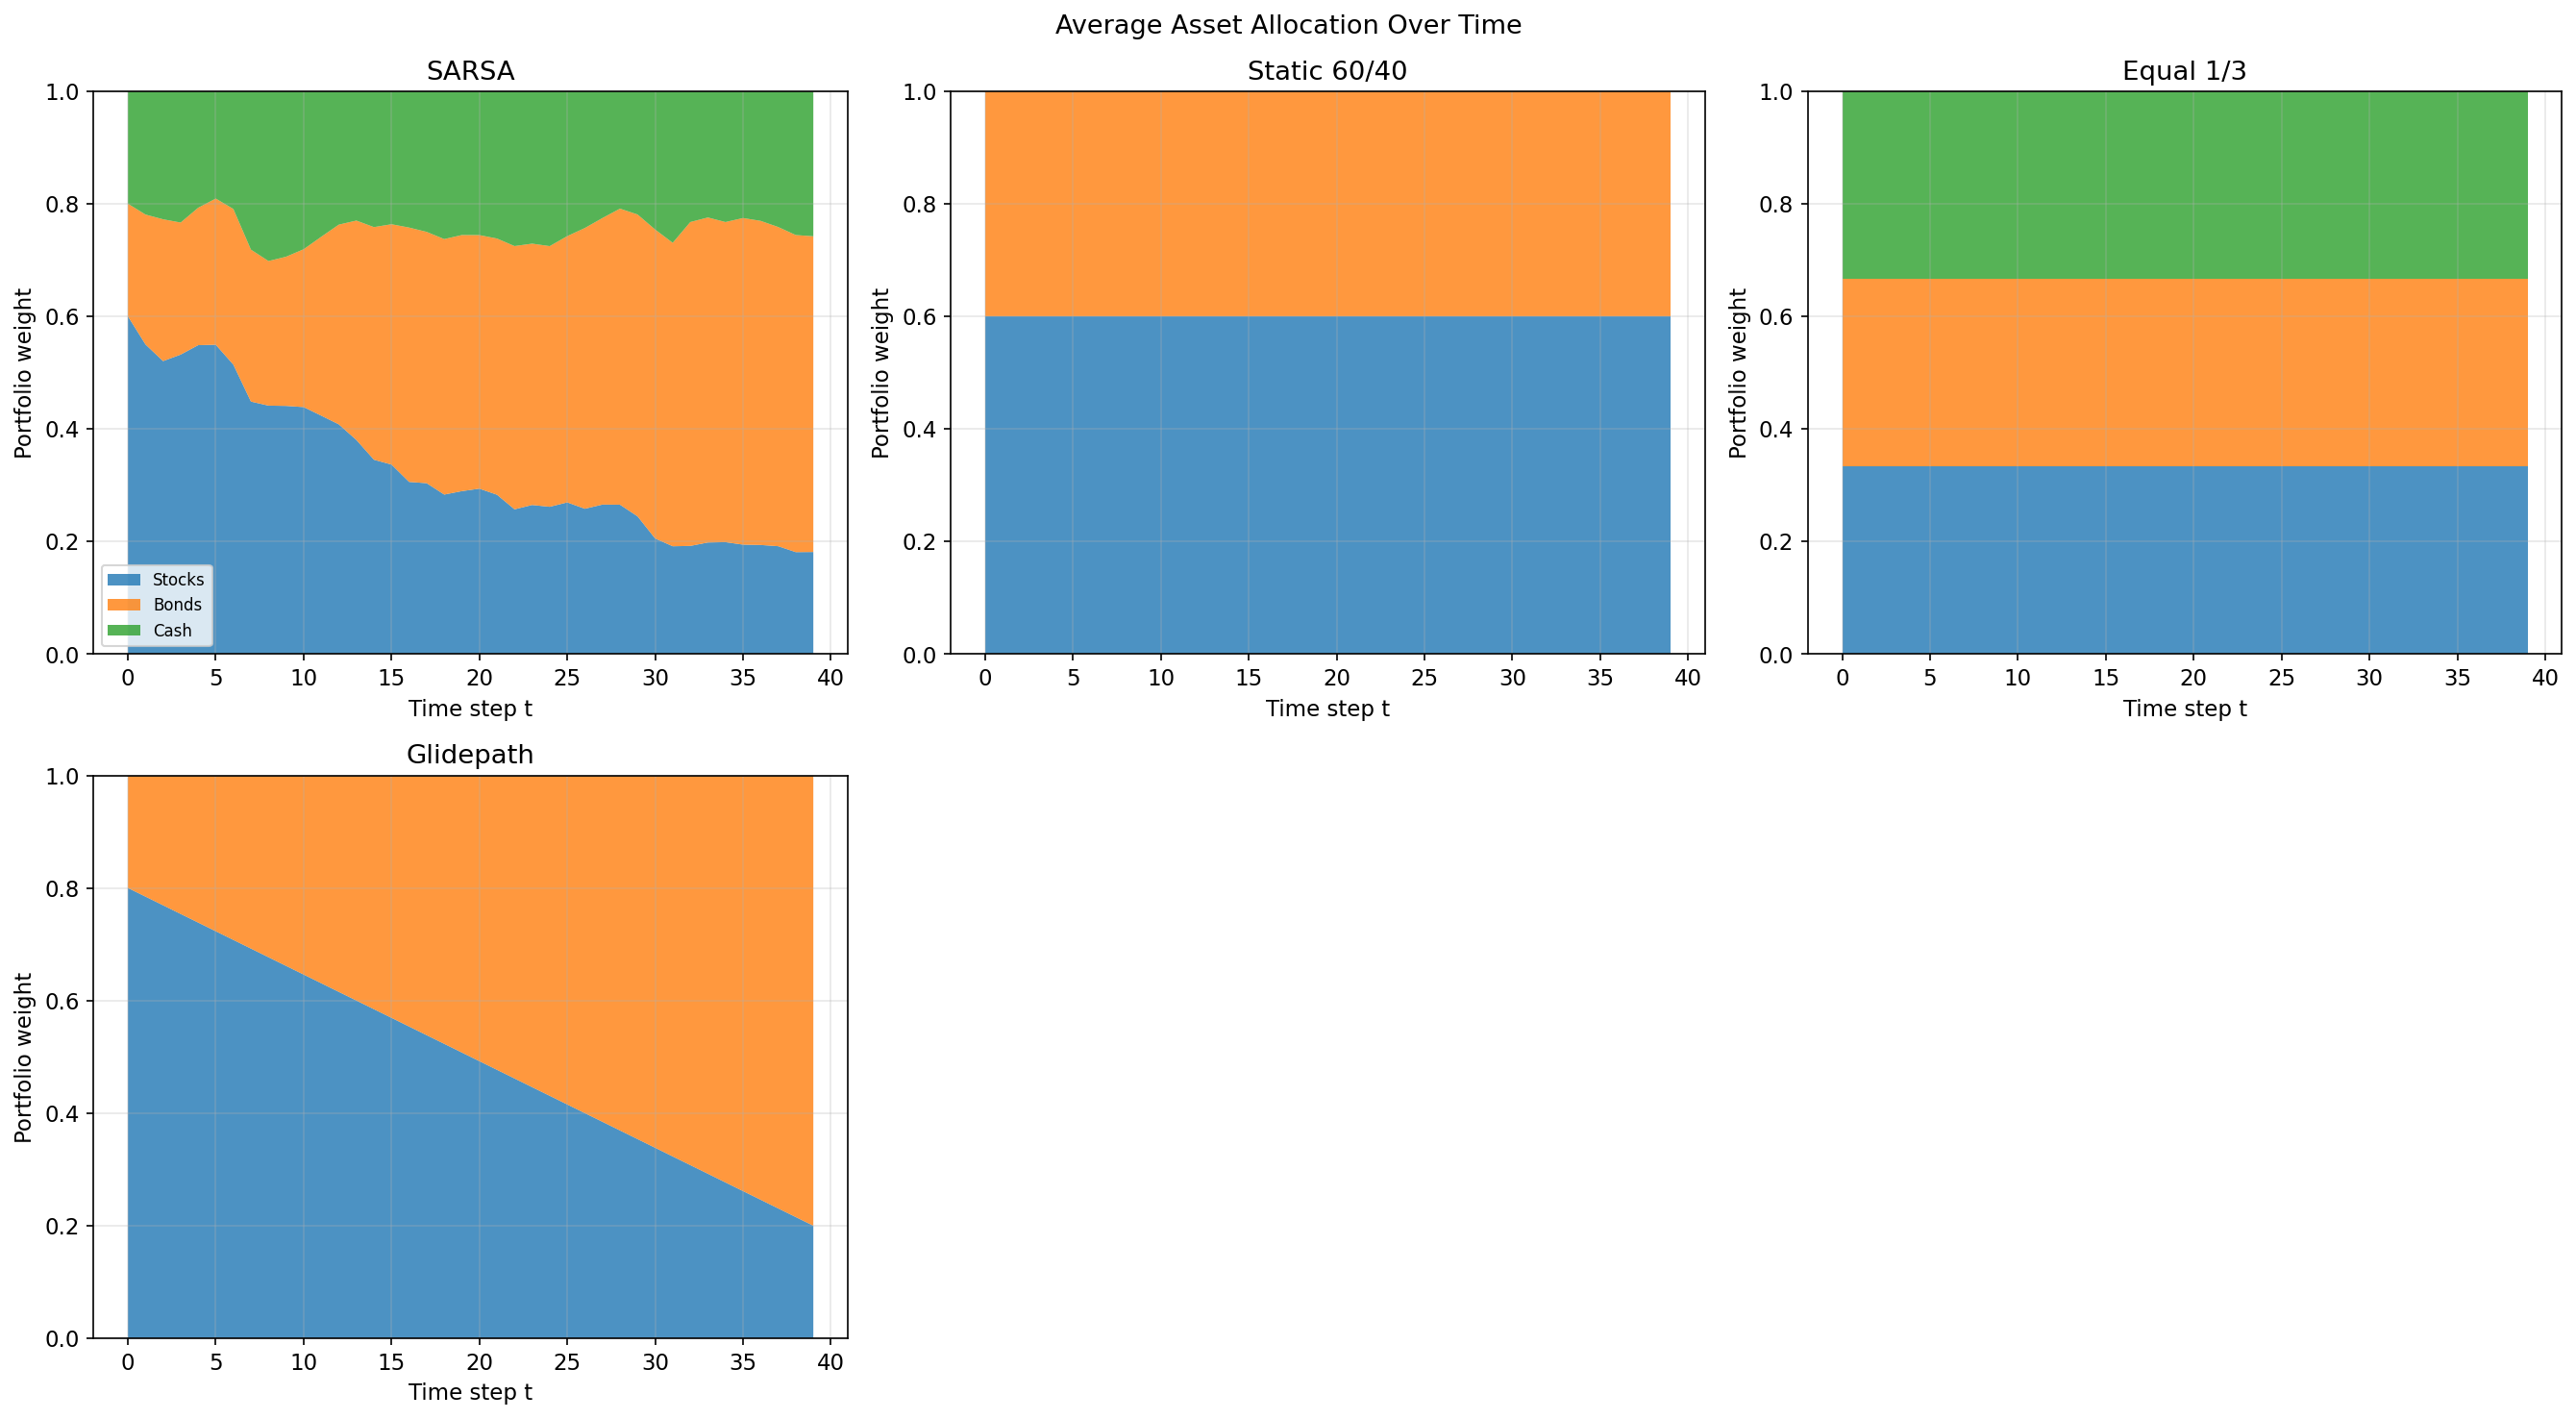
\includegraphics[width=0.95\textwidth]{phase3/plots/allocation_stacks.png}
  \caption{Average portfolio weights over the horizon for RL agents and baselines (stocks, bonds, cash). Linear $Q$ exhibits a smooth de-risking; DQN concentrates in stocks; PPO and SARSA use substantial cash early before reallocating.}
  \label{fig:alloc}
\end{figure}

Phase~2 DP on the small grid yields mean utility about $-0.95$ and mean terminal wealth $\approx 88.5$ on comparable baseline simulations; see \citep{projectreport}. Scaling to Phase~3 changes absolute utility levels but preserves the ranking insight: \textbf{optimizing consumption timing} under CRRA need not maximize terminal wealth. RL agents rank above baselines on $\mathbb{E}[U]$ while exhibiting lower $\mathbb{E}[W_T]$.

\section{Discussion}

Linear $Q$ and SARSA produce interpretable, highly state-dependent heatmaps when consumption and stock shares are plotted against time and wealth; explicit feature interactions help. DQN achieves the best mean utility here with a nearly stationary aggressive policy (high equity, high consumption grid point), which is consistent with a long horizon and positive equity premium in the simulator. PPO shows strong time structure (e.g., cash-heavy early periods) but underperforms DQN on $\mathbb{E}[U]$ in our runs. Off-policy value methods outperform on-policy counterparts (Linear $Q$ vs SARSA; DQN vs PPO) on this metric, though SARSA offers conservative tail behavior (higher $\min W_T$ than DQN).

\textbf{Limitations.} The joint discrete action space is inefficient; factored actions or continuous control would improve exploration. Regimes and income are stylized; transaction costs, taxes, and empirical calibration are omitted. Training seed and agent order affect reproducibility when a shared random stream is used across sequential training runs.

\section{Conclusion}

Exact DP validates the economic problem and clarifies objectives, but a modest increase in problem size makes full tabulation prohibitive. With careful reward design and training infrastructure, four standard RL algorithms learn policies that dominate common investment heuristics on discounted CRRA welfare. The gap between terminal wealth and utility underscores the importance of aligning computational objectives with household welfare. Future work includes continuous actions, larger asset menus, and estimation from market and panel data.

\section*{Acknowledgments}

Course project for CME~241 (Stanford, Winter~2026). Code and configuration are available in the repository under \texttt{project/phase3/}.

\bibliographystyle{plainnat}
\begin{thebibliography}{xx}

\bibitem[Judd(1998)]{judd1998numerical}
Judd, K.~L. (1998).
\newblock \emph{Numerical Methods in Economics}.
\newblock MIT Press.

\bibitem[Jiang et~al.(2017)]{jiang2017cryptocurrency}
Jiang, Z., Liang, J., and Li, L. (2017).
\newblock Cryptocurrency portfolio management with deep reinforcement learning.
\newblock In \emph{Intelligent Systems Conference}.

\bibitem[Merton(1969)]{merton1969lifetime}
Merton, R.~C. (1969).
\newblock Lifetime portfolio selection under uncertainty: The continuous-time case.
\newblock \emph{Journal of Economic Theory}, 3(4):373--413.

\bibitem[Mnih et~al.(2015)]{mnih2015human}
Mnih, V., Kavukcuoglu, K., Silver, D., et~al. (2015).
\newblock Human-level control through deep reinforcement learning.
\newblock \emph{Nature}, 518(7540):529--533.

\bibitem[Samuelson(1969)]{samuelson1969lifetime}
Samuelson, P.~A. (1969).
\newblock Lifetime portfolio selection by dynamic stochastic programming.
\newblock \emph{The Review of Economics and Statistics}, 51(3):239--246.

\bibitem[Schulman et~al.(2017)]{schulman2017proximal}
Schulman, J., Wolski, F., Dhariwal, P., Radford, A., and Klimov, O. (2017).
\newblock Proximal policy optimization algorithms.
\newblock \emph{arXiv:1707.06347}.

\bibitem[Sutton and Barto(2018)]{sutton2018reinforcement}
Sutton, R.~S. and Barto, A.~G. (2018).
\newblock \emph{Reinforcement Learning: An Introduction}.
\newblock MIT Press, 2nd edition.

\bibitem[Wang et~al.(2016)]{wang2016dueling}
Wang, Z., Schaul, T., Hessel, M., van Hasselt, H., Lanctot, M., and de Freitas, N. (2016).
\newblock Dueling network architectures for deep reinforcement learning.
\newblock In \emph{ICML}.

% \bibitem[Project report(2026)]{projectreport}
% Flanagan, P., Zhang, J., and Xue, J. (2026).
% \newblock Lifecycle dynamic asset allocation: DP and RL approaches.
% \newblock Internal project report, \texttt{project/report.md}.

\end{thebibliography}

\end{document}
